\documentclass[10pt]{article}

\usepackage[utf8]{inputenc}
\usepackage[T1]{fontenc}
\usepackage[spanish]{babel}
\usepackage[table]{xcolor}
\usepackage{adjustbox}
\usepackage{amsfonts}
\usepackage{amsmath}
\usepackage{amssymb}
\usepackage{array}
\usepackage{booktabs}
\usepackage{caption}
\usepackage{enumitem}
\usepackage{fancyhdr}
\usepackage{float}
\usepackage{fontspec}
\usepackage{geometry}
\usepackage{graphicx}
\usepackage{hyperref}
\usepackage{lipsum}
\usepackage{mathtools}
\usepackage{multirow}
\usepackage[numbers]{natbib}
\usepackage{parskip}
\usepackage{ragged2e}
\usepackage{setspace}
\usepackage{siunitx}
\usepackage{subcaption}
\usepackage{soul}
\usepackage{tabularx}
\usepackage{tcolorbox}
\usepackage{threeparttable}
\usepackage{tikz}
\usepackage{titlesec}
\usepackage{url}

\setstretch{0.7}
\titlespacing*{\section}{0pt}{*0.25}{*0.25}
\titlespacing*{\subsection}{0pt}{*0.25}{*0.25}
\setlength{\parskip}{0.2cm}
\setlength{\parindent}{0pt}
\setlength{\textfloatsep}{8pt plus 2pt minus 2pt}
\setlength{\floatsep}{6pt plus 2pt minus 2pt}
\setlength{\intextsep}{6pt plus 2pt minus 2pt}
\renewcommand{\topfraction}{0.95}
\renewcommand{\bottomfraction}{0.85}
\renewcommand{\textfraction}{0.05}
\renewcommand{\floatpagefraction}{0.85}
\raggedbottom

\captionsetup[figure]{labelfont=bf, skip=4pt}
\captionsetup[table]{labelfont=bf, skip=4pt}
\captionsetup{labelformat=simple, labelsep=period, belowskip=0pt}
\renewcommand{\tablename}{Cuadro}
\hypersetup{
	hidelinks,
	pdfborder={0 0 0}
}
\newcommand{\cuadroref}[1]{\hyperref[#1]{Cuadro~\ref*{#1}}}
\newcommand{\figuraref}[1]{\hyperref[#1]{Figura~\ref*{#1}}}
\newcommand{\figurasrangeref}[2]{\hyperref[#1]{Figuras~\ref*{#1}--\ref*{#2}}}

\geometry{
	a4paper,
	left=20mm,
	right=20mm,
	top=25mm,
	bottom=25mm
}

\pagestyle{fancy}
\fancyhf{}
\fancyhead[L]{UBA | FCE}
\fancyhead[R]{Informe Final}
\fancyfoot[C]{\thepage}
\renewcommand{\headrulewidth}{0.4pt}
\renewcommand{\footrulewidth}{0pt}

\begin{document}

		\begin{center}
			\Large Universidad de Buenos Aires \\[0.2cm]
			\large Facultad de Ciencias Económicas \\[0.2cm]
			Escuela de Estudios de Posgrado \\[0.4cm]
			\Large \textbf{ANÁLISIS PREDICTIVO DE TARIFAS DE VIAJES EN LA PLATAFORMA UBER: APLICACIONES DE MODELOS DE APRENDIZAJE AUTOMÁTICO EN INTELIGENCIA DE NEGOCIOS} \\[0.4cm]
			\textbf{Informe Final} \\[0.4cm]
			\normalsize \textbf{DOCENTE:} FRANCO MASTELLI  \\[0.6cm]
			\Large \textbf{ASIGNATURA:} INTELIGENCIA DE NEGOCIOS \\[0.5cm]

			\normalsize \textbf{ALUMNO:} JULIÁN DELGADILLO MARÍN \\[0.2cm]
			\textbf{POSGRADO:} MAESTRÍA EN ECONOMÍA APLICADA \\[0.4cm]
			\textbf{FECHA:} \today
			\vspace*{1cm}
		\end{center}

	\begin{center}
		\section*{Resumen}
	\end{center}

	\justify
	El presente trabajo desarrolla un ejercicio aplicado de Inteligencia de Negocios orientado a la estimación de tarifas de viajes Uber en la ciudad de Nueva York, a partir de información geográfica, temporal y operativa disponible en el dataset. Se comparan modelos lineales, modelos de ensamble y redes neuronales densas para predecir la tarifa observada (\texttt{fare\_amount}).

	El modelo lineal ampliado muestra una asociación positiva entre distancia y tarifa, con un coeficiente cercano a 2 USD por kilómetro y un nivel de explicación de 70.6\%. En la evaluación final sobre el mismo conjunto de prueba oficial, la red neuronal con cuatro capas ocultas obtuvo el menor error (RMSE = 1.9149; MAE = 1.2327), seguida por \textit{Gradient Boosting} (RMSE = 1.9429; MAE = 1.2753). En conjunto, el análisis sugiere que la distancia recorrida sigue siendo el predictor central, mientras que las variables temporales, la cantidad de pasajeros y las coordenadas geográficas aportan información adicional para mejorar la precisión. El estudio ofrece una base reproducible para ejercicios de analítica descriptiva, modelado predictivo y evaluación de desempeño en contextos de movilidad urbana.

	\vspace{0.3cm}
	\noindent\textbf{Palabras clave:} Inteligencia de Negocios, Aprendizaje Automático, Regresión Lineal, Modelos de Ensamble, Redes Neuronales, Uber, Predicción de Tarifas, Análisis de Datos, Movilidad Urbana.

		\vspace{1cm}

	% =============================
	% SECCIONES DEL INFORME
	% =============================

	\section{Introducción}

	En el presente informe se desarrolla un ejercicio aplicado de Inteligencia de Negocios orientado al análisis y predicción de tarifas de viajes de \textit{Uber} en la ciudad de Nueva York. A partir de un conjunto de datos con información georreferenciada de origen y destino, y con la tarifa final observada para cada trayecto, se estudia la relación entre la distancia recorrida y el monto cobrado (\texttt{fare\_amount}).

	El trabajo combina limpieza de datos, análisis exploratorio, ingeniería de variables y modelado predictivo. En particular, se calcula la distancia geodésica entre puntos de origen y destino mediante la fórmula de Haversine, se aplican filtros para remover observaciones inconsistentes o atípicas, y se construye una muestra final para entrenamiento y evaluación de modelos.

	Sobre esta base se comparan distintos enfoques de aprendizaje supervisado: modelos lineales tradicionales, regresión regularizada, métodos de ensamble basados en árboles y redes neuronales artificiales. La comparación se realiza sobre conjuntos de prueba utilizando métricas de error como RMSE y MAE, con el propósito de evaluar la capacidad predictiva de cada alternativa y discutir el equilibrio entre precisión, complejidad e interpretabilidad.

	De este modo, el informe busca mostrar cómo un flujo reproducible de análisis de datos puede transformar registros transaccionales en evidencia útil para la estimación de tarifas y la toma de decisiones en contextos de Inteligencia de Negocios.

	\section{Objetivos}

	\subsection{Objetivo general}

	Analizar y predecir la variable \texttt{fare\_amount} a partir de la distancia recorrida estimada y variables complementarias del viaje, utilizando herramientas de Inteligencia de Negocios y Aprendizaje Automático para comparar modelos lineales, de ensamble y neuronales en la estimación de tarifas de \textit{Uber} en la ciudad de Nueva York.

	\subsection{Objetivos específicos}

	\begin{enumerate}[label=\textbf{O\arabic*.}]
		\item Realizar un análisis exploratorio de datos para describir la estructura, distribución y calidad del conjunto de datos, identificando valores faltantes, inconsistencias y observaciones atípicas.

		\item Calcular la distancia geodésica entre los puntos de origen y destino mediante la fórmula de Haversine, construyendo la variable \texttt{distance\_km} como insumo principal del análisis.

		\item Aplicar criterios de limpieza y filtrado sobre las variables \texttt{fare\_amount} y \texttt{distance\_km}, con el propósito de mejorar la coherencia del dataset utilizado en la modelización.

		\item Dividir el conjunto de datos en muestras de entrenamiento y prueba bajo un esquema reproducible, utilizando el número de documento del estudiante como \texttt{random\_state}.

		\item Ajustar modelos de regresión lineal y regresión regularizada para establecer una línea base de desempeño e interpretar la relación entre las variables disponibles y la tarifa.

		\item Entrenar modelos de ensamble, específicamente \textit{Random Forest} y \textit{Gradient Boosting}, para evaluar mejoras predictivas frente a los enfoques lineales.

		\item Diseñar y evaluar distintas arquitecturas de redes neuronales artificiales para explorar su desempeño en la estimación de tarifas de viaje.

		\item Comparar el desempeño de todos los modelos sobre datos de prueba mediante las métricas RMSE y MAE, identificando el modelo con mejor capacidad predictiva.

		\item Discutir los resultados obtenidos considerando la precisión, la interpretabilidad y la utilidad de los modelos en un contexto de Inteligencia de Negocios.
	\end{enumerate}

	\section{Marco Teórico}
	\label{sec:marco-teorico}

	\subsection{Inteligencia de Negocios y análisis predictivo}
	La \textit{Inteligencia de Negocios} (BI) integra procesos, datos y herramientas analíticas para transformar información operativa en conocimiento accionable. En su vertiente predictiva, BI incorpora modelos estadísticos y de \textit{machine learning} para estimar variables de interés y apoyar la toma de decisiones bajo incertidumbre. En problemas de tarificación, el objetivo típico es modelar la relación entre variables explicativas (p.\,ej., distancia, tiempo, contexto geográfico) y la tarifa observada, buscando un compromiso entre precisión, interpretabilidad y costo computacional.

	\subsection{Modelado de datos y toma de decisiones}
	Desde la perspectiva de BI, el modelado cumple dos roles complementarios: (i) descriptivo/explicativo, al cuantificar asociaciones e interpretar relaciones entre variables; y (ii) predictivo, al minimizar el error en datos no vistos. En ambos casos, la calidad del dato (limpieza, tratamiento de atípicos, ingeniería de características) es determinante para evitar sesgos y mejorar la \textit{generalización}. La evaluación fuera de muestra (\textit{holdout} o validación cruzada) es el mecanismo estándar para estimar el rendimiento esperado.

	\subsection{Regresión lineal (MCO) e interpretación}
	El modelo lineal con Mínimos Cuadrados Ordinarios (MCO) asume
	\[
	y = \beta_0 + \mathbf{x}^\top\boldsymbol{\beta} + \varepsilon,\qquad \mathbb{E}[\varepsilon|\mathbf{x}]=0,
	\]
	y estima los parámetros resolviendo
	\[
	\hat{\boldsymbol{\beta}}_{\text{OLS}}
	= \arg\min_{\boldsymbol{\beta}} \; \sum_{i=1}^{n}\bigl(y_i - \beta_0 - \mathbf{x}_i^\top\boldsymbol{\beta}\bigr)^2.
	\]
	Sus ventajas son la interpretabilidad (coeficientes como efectos marginales) y la disponibilidad de inferencia clásica (errores estándar, pruebas $t$). Sus limitaciones aparecen ante relaciones no lineales, colinealidad y presencia de \textit{outliers}.

	\subsection{Regularización LASSO}
	Para controlar el sobreajuste y comparar la estabilidad de un modelo lineal regularizado frente a una regresión lineal tradicional, la regularización $L_1$ (LASSO) incorpora una penalización a la magnitud de los coeficientes:
	\[
	\hat{\boldsymbol{\beta}}_{\text{LASSO}}
	= \arg\min_{\boldsymbol{\beta}} \left\{
	\sum_{i=1}^{n}\bigl(y_i-\beta_0-\mathbf{x}_i^\top\boldsymbol{\beta}\bigr)^2
	\;+\; \lambda \lVert \boldsymbol{\beta}\rVert_1
	\right\},
	\]
	donde $\lambda\ge 0$ controla la fuerza de la penalización. En modelos con múltiples predictores, LASSO puede llevar algunos coeficientes a cero y producir soluciones más parsimoniosas. En este trabajo, donde el énfasis está puesto en la relación entre distancia y tarifa, su utilidad principal es servir como contraste regularizado frente al modelo OLS. El hiperparámetro $\lambda$ se selecciona típicamente por validación cruzada, optimizando una métrica como RMSE o MAE.

	\subsection{Modelos de ensamble: Random Forest y Gradient Boosting}
	\paragraph{Random Forest (RF).} Combina múltiples árboles de decisión entrenados sobre \textit{bootstraps} de los datos y subconjuntos aleatorios de variables. La predicción final promedia las predicciones individuales:

	\[
	\hat{f}_{\text{RF}}(\mathbf{x})=\frac{1}{B}\sum_{b=1}^{B} T_b(\mathbf{x}),
	\]

	lo que reduce la varianza respecto de un árbol único y permite aproximar relaciones no lineales sin imponer una forma funcional rígida. Sus hiperparámetros clave incluyen la profundidad máxima, el número de árboles y los criterios de división.

	\paragraph{Gradient Boosting (GB).} Construye aditivamente un ensamble de árboles poco profundos, ajustando en cada etapa un nuevo árbol a los \textit{residuales} del ensamble previo:

	\begin{align}
		\hat{f}_0(\mathbf{x}) &=
		\arg\min_c \sum_i L(y_i,c), \\[2pt]
		\hat{f}_m(\mathbf{x}) &=
		\hat{f}_{m-1}(\mathbf{x})
		+ \nu \, h_m(\mathbf{x}).
	\end{align}


	donde $h_m$ es el árbol ``débil'' de la etapa $m$, $L(\cdot)$ es la pérdida (p.\,ej., cuadrática) y $\nu\in(0,1]$ el \textit{learning rate}. GB suele lograr buen desempeño predictivo con árboles más someros, a costa de una mayor sensibilidad a hiperparámetros como el número de etapas, la profundidad y la tasa de aprendizaje. En este informe, ambos métodos se utilizan principalmente para evaluar si una especificación no lineal mejora la predicción obtenida con los modelos lineales.

	\subsection{Redes neuronales densas (perceptrón multicapa)}
	Las redes densas aproximan funciones mediante composiciones de transformaciones afines y no lineales:

	\begin{align}
		\hat{y}
		&= f(\mathbf{x};\boldsymbol{\theta})  \\[2pt]
		&= \mathbf{W}_L \,
		\sigma\!\Bigl(
		\mathbf{W}_{L-1}\,
		\sigma\!\bigl(\cdots
		\sigma(\mathbf{W}_1 \mathbf{x}+\mathbf{b}_1)
		\bigr)
		+\mathbf{b}_{L-1}
		\Bigr)
		+ \mathbf{b}_L.
	\end{align}

	donde $\sigma(\cdot)$ es una activación (p.\,ej., ReLU) y $\boldsymbol{\theta}$ agrupa pesos y sesgos. Para regresión, la pérdida típica es el error cuadrático medio

	\[
	\mathcal{L}(\boldsymbol{\theta})=\frac{1}{n}\sum_{i=1}^{n}\bigl(y_i - f(\mathbf{x}_i;\boldsymbol{\theta})\bigr)^2,
	\]

	optimizándose por descenso por gradiente (p.\,ej., Adam) con técnicas de regularización (early stopping, dropout, penalizaciones $L_1/L_2$). Su fortaleza reside en modelar relaciones altamente no lineales; su debilidad, en la menor interpretabilidad y en la sensibilidad a la configuración.

	\subsection{Sesgo–varianza, métricas y selección de modelo}
	El desempeño de generalización resulta del equilibrio sesgo--varianza. Modelos simples, como los lineales, tienden a mayor sesgo y menor varianza; modelos más flexibles, como ensambles y redes neuronales, pueden reducir el sesgo, aunque también aumentan el riesgo de sobreajuste si no se controlan adecuadamente. Para comparar los modelos se utilizan métricas de error en datos de prueba, principalmente \textit{RMSE} y \textit{MAE}. En los modelos lineales también se reportan medidas de ajuste, como $R^2$, con fines descriptivos.

	\subsection{Ventajas y limitaciones comparadas}
	\begin{itemize}
		\item \textbf{OLS/LASSO}: alta interpretabilidad y base inferencial; limitados ante no linealidades fuertes o interacciones no modeladas.
		\item \textbf{RF/GB}: permiten aproximar relaciones no lineales sin imponer una especificación paramétrica rígida; requieren ajuste cuidadoso de hiperparámetros y su interpretación es menos directa que en los modelos lineales.
		\item \textbf{Redes densas}: alta flexibilidad funcional y precisión potencialmente competitiva; requieren mayor cuidado en tuning, escalado y control de sobreajuste; interpretabilidad reducida.
	\end{itemize}

	\vspace{0.5em}
	\noindent\textit{Nota.} Este marco teórico sustenta la comparación empírica desarrollada en las secciones de Metodología y Resultados, justificando la inclusión de modelos lineales, de ensamble y neuronales para el problema de predicción de tarifas.

	\section{Metodología}
	\label{sec:metodologia}

	La metodología implementada sigue un enfoque secuencial y reproducible de análisis de datos, alineado con las etapas de un proceso aplicado de Inteligencia de Negocios: lectura de datos, depuración, exploración, modelado y evaluación. El flujo general partió de 200\,000 registros originales, aplicó filtros geográficos y de tarifa, construyó la variable \texttt{distance\_km} y utilizó un dataset final de 179\,855 observaciones para la partición de entrenamiento y prueba.

	\subsection{Descripción del dataset}
	El conjunto de datos empleado corresponde al \textit{Uber NYC Dataset}, que recopila registros de viajes individuales realizados en la ciudad de Nueva York. Cada observación contiene información geográfica (coordenadas de origen y destino), temporal (fecha y hora del viaje), económica (monto de la tarifa, \texttt{fare\_amount}) y operativa, como la cantidad de pasajeros transportados.
	El archivo original contiene 200\,000 registros y siete variables. Para el modelado se utilizaron principalmente las coordenadas de origen y destino, la tarifa observada y la variable calculada \texttt{distance\_km}.

	Antes de aplicar transformaciones o filtros, se efectuó un análisis descriptivo inicial con el propósito de identificar inconsistencias, valores extremos y la distribución general de las variables. Los principales estadísticos se presentan en el \cuadroref{tab:estadisticas_iniciales}.

	\begin{table}[!htbp]
		\centering
		\caption{Estadísticas descriptivas del dataset original de viajes Uber (200{,}000 observaciones).}
		\label{tab:estadisticas_iniciales}
		\begin{adjustbox}{max width=0.95\textwidth,center}
			\begin{tabular}{lrrrrrrrr}
				\hline
				\textbf{Variable} & \textbf{count} & \textbf{mean} & \textbf{std} & \textbf{min} & \textbf{25\%} & \textbf{50\%} & \textbf{75\%} & \textbf{max} \\
				\hline
				\texttt{fare\_amount} & 200{,}000 & 11.36 & 9.90 & -52.00 & 6.00 & 8.50 & 12.50 & 499.00 \\
				\texttt{pickup\_longitude} & 200{,}000 & -72.53 & 11.44 & -1340.65 & -73.99 & -73.98 & -73.97 & 57.42 \\
				\texttt{pickup\_latitude} & 200{,}000 & 39.94 & 7.72 & -74.02 & 40.73 & 40.75 & 40.77 & 1644.42 \\
				\texttt{dropoff\_longitude} & 199{,}999 & -72.53 & 13.12 & -3356.67 & -73.99 & -73.98 & -73.96 & 1153.57 \\
				\texttt{dropoff\_latitude} & 199{,}999 & 39.92 & 6.79 & -881.99 & 40.73 & 40.75 & 40.77 & 872.70 \\
				\texttt{passenger\_count} & 200{,}000 & 1.68 & 1.39 & 0.00 & 1.00 & 1.00 & 2.00 & 208.00 \\
				\hline
			\end{tabular}
		\end{adjustbox}
	\end{table}

	Como puede observarse, las variables geográficas presentan valores fuera del rango esperado para Nueva York y la variable \texttt{fare\_amount} incluye tarifas negativas y valores extremos. Este diagnóstico inicial permitió delimitar el dominio espacial del análisis y fundamentar las decisiones de filtrado aplicadas en el preprocesamiento.

	El análisis exploratorio inicial también incluyó una revisión estadística de las variables geográficas del conjunto de datos original, con el objetivo de verificar la coherencia espacial de los registros. Se evaluaron los valores mínimos, máximos y medidas de tendencia central para las coordenadas de origen y destino.

	Los resultados, presentados en el \cuadroref{tab:rango_coordenadas}, revelan la existencia de valores extremos que no corresponden a ubicaciones dentro del área metropolitana de Nueva York. Por ejemplo, se observaron longitudes inferiores a --1300 y latitudes mayores a 1600, lo cual evidencia errores de captura o codificación en el registro de coordenadas.

	\begin{table}[!htbp]
		\centering
		\caption{Rango estadístico de las coordenadas geográficas del dataset original.}
		\label{tab:rango_coordenadas}
		\begin{adjustbox}{max width=0.95\textwidth,center}
			\begin{tabular}{lrrrr}
				\hline
				\textbf{Estadístico} & \texttt{pickup\_longitude} & \texttt{pickup\_latitude} & \texttt{dropoff\_longitude} & \texttt{dropoff\_latitude} \\
				\hline
				count & 200{,}000 & 200{,}000 & 199{,}999 & 199{,}999 \\
				mean & -72.53 & 39.94 & -72.53 & 39.92 \\
				std & 11.44 & 7.72 & 13.12 & 6.79 \\
				min & -1340.65 & -74.02 & -3356.67 & -881.99 \\
				25\% & -73.99 & 40.73 & -73.99 & 40.73 \\
				50\% & -73.98 & 40.75 & -73.98 & 40.75 \\
				75\% & -73.97 & 40.77 & -73.96 & 40.77 \\
				max & 57.42 & 1644.42 & 1153.57 & 872.70 \\
				\hline
			\end{tabular}
		\end{adjustbox}
	\end{table}

	La dispersión observada en los valores de longitud y latitud respalda la necesidad de implementar un proceso de depuración geográfica, restringiendo el análisis a los rangos válidos para la ciudad de Nueva York. Esta decisión permitió mejorar la coherencia espacial de los datos y la consistencia del cálculo posterior de distancias.

	\subsection{Procesamiento y limpieza de datos}

	El procesamiento se desarrolló en tres etapas principales: depuración de coordenadas, cálculo de distancia mediante la fórmula de Haversine y filtrado de registros inválidos o extremos en \texttt{fare\_amount} y \texttt{distance\_km}. Sobre los registros retenidos se calculó la distancia geodésica entre origen y destino mediante:

	\begin{figure}[!htbp]
		\centering
		\[
		d = 2R\, \arcsin\!\left(
		\sqrt{
			\sin^2\!\left(\frac{\Delta\varphi}{2}\right)
			+ \cos(\varphi_1)\cos(\varphi_2)
			\sin^2\!\left(\frac{\Delta\lambda}{2}\right)
		}
		\right)
		\]
		\caption{Fórmula del semiverseno (Haversine) para el cálculo de distancias geodésicas.}
		\label{eq:haversine}
	\end{figure}

	donde $R=6371$ km es el radio medio de la Tierra. Este paso permitió generar la variable \texttt{distance\_km}, que se utiliza como predictor principal del modelo de tarifas.

	Durante esta etapa se descartaron 4\,353 registros, equivalentes al 2.18\,\% del conjunto inicial, conservando 195\,647 observaciones con coordenadas válidas y distancia calculada. El resumen de esta depuración se presenta en el \cuadroref{tab:depuracion_distance}.

	\begin{table}[!htbp]
		\centering
		\caption{Resumen del proceso de depuración y creación de la variable \texttt{distance\_km}.}
		\label{tab:depuracion_distance}
		\begin{tabular}{lr}
			\hline
			\textbf{Descripción} & \textbf{Valor} \\
			\hline
			Registros originales & 200{,}000 \\
			Registros válidos & 195{,}647 \\
			Registros eliminados & 4{,}353 (2.18\%) \\
			\hline
			\textbf{Variable analizada} & \texttt{distance\_km} \\
			\hline
			count & 195{,}647 \\
			mean & 3.31 \\
			std & 3.58 \\
			min & 0.00 \\
			25\% & 1.26 \\
			50\% (mediana) & 2.16 \\
			75\% & 3.91 \\
			max & 41.23 \\
			\hline
		\end{tabular}
	\end{table}

	La distancia media estimada fue de aproximadamente 3.3\,km, con una dispersión de 3.6\,km. El rango intercuartílico (1.26–3.91\,km) sugiere predominio de trayectos urbanos de corta o media distancia.

	Una vez finalizada la depuración espacial y el cálculo de las distancias, se aplicó un filtrado adicional a la variable \texttt{fare\_amount} para eliminar valores negativos, nulos o excesivamente altos. Este procedimiento permitió obtener una distribución más estable para el análisis posterior.

	El \cuadroref{tab:fare_filtrada} presenta un resumen estadístico de la variable \texttt{fare\_amount} después del proceso de filtrado. Se observa que el número total de registros válidos se redujo a 193{,}301, con una tarifa máxima de USD 51.90. La media resultante (USD 10.72) y la mediana (USD 8.50) reflejan la predominancia de trayectos de corta y mediana distancia.

	\begin{table}[!htbp]
		\centering
		\caption{Estadísticas descriptivas de la variable \texttt{fare\_amount} después del filtrado.}
		\label{tab:fare_filtrada}
		\begin{tabular}{lr}
			\hline
			\textbf{Descripción} & \textbf{Valor} \\
			\hline
			Registros luego del filtrado & 193{,}301 \\
			Tarifa máxima después del filtrado & USD 51.90 \\
			\hline
			count & 193{,}301 \\
			mean & 10.72 \\
			std & 7.80 \\
			min & 0.01 \\
			25\% & 6.00 \\
			50\% (mediana) & 8.50 \\
			75\% & 12.50 \\
			max & 51.90 \\
			\hline
		\end{tabular}
	\end{table}

	Este ajuste reduce la influencia de valores extremos y deja una distribución más adecuada para el análisis exploratorio y los modelos predictivos.

	La \figuraref{fig:distribucion_fare_filtrado} muestra la distribución de frecuencias de \texttt{fare\_amount} en el dataset filtrado. Se observa una clara asimetría hacia la derecha, característica de variables de tipo monetario, donde la mayoría de los registros se concentran entre 5 y 15 USD, correspondientes a viajes de corta o media distancia. Los valores por encima de 30 USD son escasos y reflejan desplazamientos más largos o hacia zonas periféricas.

	\begin{figure}[!htbp]
		\centering
		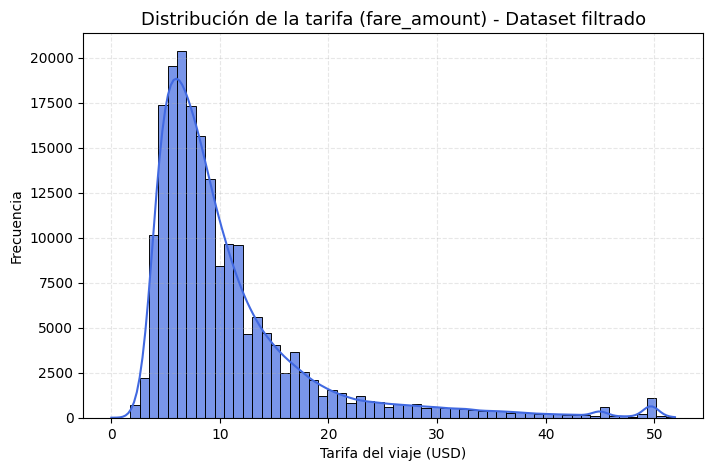
\includegraphics[width=0.74\textwidth,height=0.30\textheight,keepaspectratio]{../figures/9.png}
		\caption{Distribución de la variable \texttt{fare\_amount} (tarifa del viaje en USD) después del filtrado del dataset. Se observa una distribución asimétrica hacia la derecha con la mayoría de los valores concentrados entre 5 y 15 USD.}
		\label{fig:distribucion_fare_filtrado}
	\end{figure}

	En una etapa posterior se evaluó la presencia de valores atípicos en las variables \texttt{fare\_amount} y \texttt{distance\_km}. Para ello, se aplicó el criterio del rango intercuartílico (IQR, por sus siglas en inglés), que permite identificar observaciones alejadas del rango central de la distribución.

	El \cuadroref{tab:outliers_iqr_transpuesta} resume los resultados de esta detección, indicando la cantidad y el porcentaje de registros ubicados fuera de los límites teóricos establecidos por el IQR. Se observa que aproximadamente un 5.6\% de las observaciones en ambas variables se ubicaban fuera de dichos rangos.

	\begin{table}[!htbp]
		\centering
		\caption{Detección de valores atípicos mediante el rango intercuartílico (IQR).}
		\label{tab:outliers_iqr_transpuesta}
		\begin{adjustbox}{max width=0.95\textwidth,center}
			\begin{tabular}{lcc}
				\hline
				\textbf{Descripción} & \texttt{fare\_amount} & \texttt{distance\_km} \\
				\hline
				Observaciones fuera del rango IQR & 10{,}966 & 10{,}807 \\
				Porcentaje del total & 5.67\% & 5.59\% \\
				Rango teórico (IQR) & [-7.00, 25.50] & [-3.89, 8.95] \\
				\hline
			\end{tabular}
		\end{adjustbox}
	\end{table}

	Estos resultados muestran la presencia de un grupo acotado de registros extremos que podía afectar las medidas de tendencia central, dispersión y correlación. Por ello, se procedió a su exclusión en el dataset final de modelado.

	El filtrado formal se aplicó sobre ambas variables de manera conjunta, preservando los registros comprendidos entre los límites \( Q1 - 2.0 \times IQR \) y \( Q3 + 2.0 \times IQR \), con límite inferior truncado en cero cuando correspondía por tratarse de variables no negativas.

	El \cuadroref{tab:iqr_filtrado} resume los resultados del proceso de filtrado y su efecto sobre la correlación entre ambas variables. Se observa que el filtrado removió 13\,446 registros, equivalentes al 6.96\% del conjunto previo, reduciendo la muestra a 179\,855 observaciones. A pesar de esta depuración, la correlación de Pearson entre \texttt{fare\_amount} y \texttt{distance\_km} se mantuvo alta (0.821), lo que respalda el uso de la distancia como predictor principal.

	\begin{table}[!htbp]
		\centering
		\caption{Resumen del filtrado mediante el método IQR y su efecto sobre la correlación.}
		\label{tab:iqr_filtrado}
		\begin{adjustbox}{max width=0.95\textwidth,center}
			\begin{tabular}{lcc}
				\hline
				\textbf{Descripción} & \texttt{fare\_amount} & \texttt{distance\_km} \\
				\hline
				Límite inferior aplicado & 0.00 & 0.00 \\
				Límite superior aplicado & 25.50 & 8.95 \\
				Q1 (25\%) & 6.00 & 1.25 \\
				Q3 (75\%) & 12.50 & 3.82 \\
				IQR & 6.50 & 2.57 \\
				\hline
				Registros antes del filtrado & \multicolumn{2}{c}{193{,}301} \\
				Registros después del filtrado & \multicolumn{2}{c}{179{,}855} \\
				Registros removidos (\%) & \multicolumn{2}{c}{13{,}446 (6.96\%)} \\
				\hline
				Correlación Pearson (\texttt{fare\_amount} vs \texttt{distance\_km}) & \multicolumn{2}{c}{} \\
				\hspace{1em} Antes del filtrado & \multicolumn{2}{c}{0.875} \\
				\hspace{1em} Después del filtrado & \multicolumn{2}{c}{0.821} \\
				\hline
			\end{tabular}
		\end{adjustbox}
	\end{table}

	Este resultado sugiere que la eliminación de valores atípicos reduce la influencia de observaciones extremas sin modificar de forma sustancial la relación principal entre distancia y tarifa. Así, el dataset depurado constituye la base para los análisis exploratorios y los modelos predictivos posteriores.

	Para cuantificar el efecto del filtrado IQR sobre la distribución de las tarifas, se realizó una comparación estadística antes y después de eliminar los valores extremos. El \cuadroref{tab:fareamount_antes_despues} resume los principales estadísticos descriptivos.

	En términos prácticos, tras el filtrado se eliminó el 6.9\% de los registros más extremos, reduciendo el valor máximo de 51.9 USD a 25.5 USD. Asimismo, el desvío estándar pasó de 7.80 a 4.36 USD, indicando una mayor homogeneidad en los valores retenidos.

	\begin{table}[!htbp]
		\centering
		\caption{Comparación estadística de la variable \texttt{fare\_amount} antes y después del filtrado IQR.}
		\label{tab:fareamount_antes_despues}
		\begin{adjustbox}{max width=0.95\textwidth,center}
			\begin{tabular}{lcc}
				\hline
				\textbf{Estadístico} & \textbf{Antes del filtrado} & \textbf{Después del filtrado} \\
				\hline
				count & 193{,}301 & 179{,}855 \\
				mean & 10.72 & 9.06 \\
				std & 7.80 & 4.36 \\
				min & 0.01 & 0.01 \\
				25\% & 6.00 & 5.70 \\
				50\% (mediana) & 8.50 & 8.00 \\
				75\% & 12.50 & 11.30 \\
				max & 51.90 & 25.50 \\
				\hline
			\end{tabular}
		\end{adjustbox}
	\end{table}

	La \figuraref{fig:fare_amount_antes_despues} muestra el efecto gráfico del filtrado: la distribución posterior es más compacta y reduce el peso de la cola derecha asociada con tarifas elevadas.

	\begin{figure}[!htbp]
		\centering
		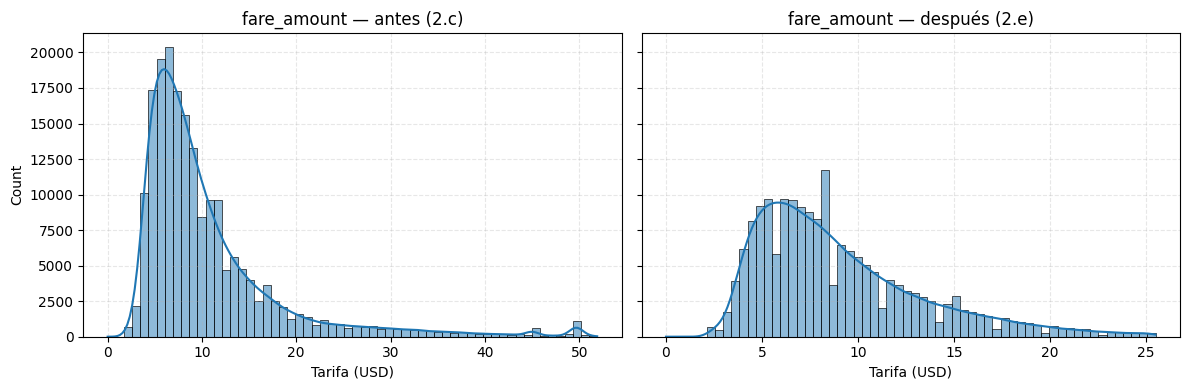
\includegraphics[width=0.82\textwidth,height=0.30\textheight,keepaspectratio]{../figures/14.png}
		\caption{Comparación de la distribución de la variable \texttt{fare\_amount} antes y después del filtrado IQR. Se observa una reducción significativa de valores extremos y una distribución más concentrada tras la depuración.}
		\label{fig:fare_amount_antes_despues}
	\end{figure}

	La \figuraref{fig:boxplot_fare_filtrado} muestra la concentración principal de tarifas entre 5 y 15 USD, con algunos valores aislados hacia el extremo superior.

	\begin{figure}[!htbp]
		\centering
		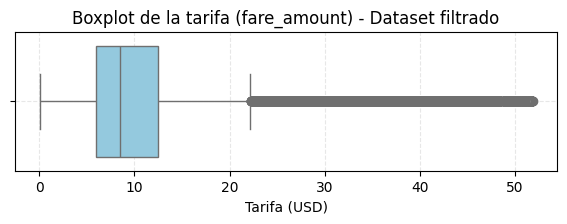
\includegraphics[width=0.66\textwidth,height=0.24\textheight,keepaspectratio]{../figures/10.png}
		\caption{Diagrama de caja (\textit{boxplot}) de la variable \texttt{fare\_amount} tras el filtrado del dataset. Se observa una concentración principal entre 5 y 15 USD, con la presencia de valores atípicos hacia el extremo superior.}
		\label{fig:boxplot_fare_filtrado}
	\end{figure}

	El efecto del proceso de depuración mediante el método IQR también puede observarse en la estructura de correlaciones entre las principales variables del conjunto de datos. En la \figuraref{fig:correlaciones_antes_despues} se comparan las matrices de correlación de Pearson calculadas antes y después del filtrado.

	Se aprecia que, tras la eliminación de valores extremos, la relación entre \texttt{fare\_amount} y \texttt{distance\_km} disminuye levemente (de $r \approx 0.88$ a $r \approx 0.82$). Esto indica que la asociación entre distancia y tarifa se mantiene alta, aunque con menor influencia de observaciones atípicas sobre la medida de correlación lineal.

	\begin{figure}[!htbp]
		\centering
		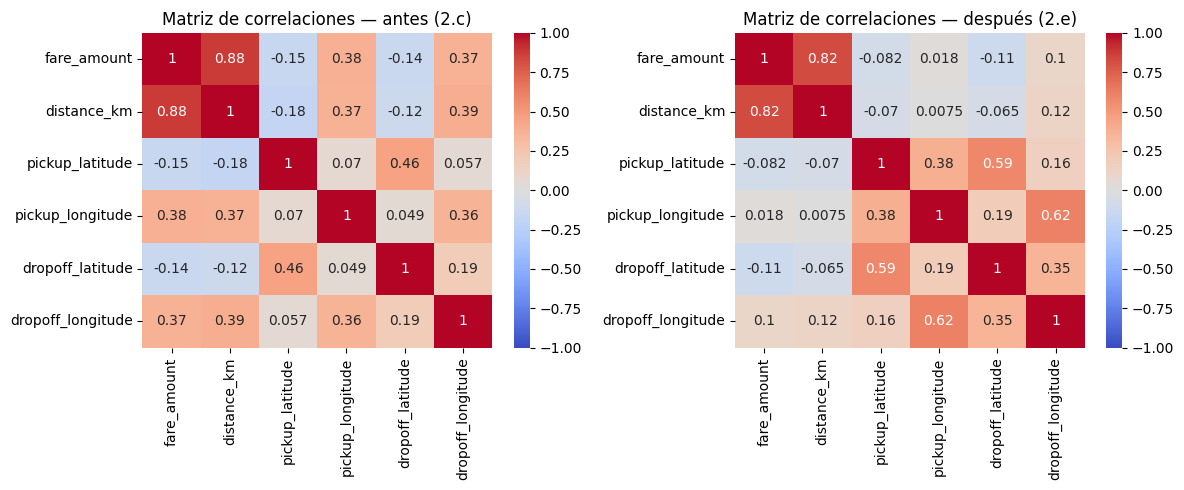
\includegraphics[width=0.82\textwidth,height=0.32\textheight,keepaspectratio]{../figures/15.png}
		\caption{Comparación de las matrices de correlación de Pearson antes y después del filtrado IQR. Se aprecia una ligera reducción en la fuerza de las correlaciones, especialmente entre \texttt{fare\_amount} y \texttt{distance\_km}, lo que refleja la eliminación de valores atípicos extremos.}
		\label{fig:correlaciones_antes_despues}
	\end{figure}

	\subsection{Análisis exploratorio de datos (EDA)}

	El EDA permitió caracterizar la estructura del dataset final y la relación entre las variables utilizadas en el modelado. Se analizaron distribuciones, correlaciones y patrones espaciales mediante:
	\begin{itemize}
		\item Mapas de dispersión, densidad y hexágonos (\textit{hexbin}) para los puntos de recogida y destino.
		\item Histogramas y diagramas de dispersión entre \texttt{fare\_amount} y \texttt{distance\_km}.
		\item Matrices de correlación de Pearson y Spearman.
	\end{itemize}

	Estos resultados se sintetizan en las \figurasrangeref{fig:uber_mapa_geografico}{fig:uber_correlaciones_spearman}, donde se observa la concentración espacial de los viajes y la asociación positiva entre distancia y tarifa.

	Una vez concluido el proceso de depuración y validación de coordenadas, se generó una representación geográfica de los puntos de origen (\textit{pickup}) y destino (\textit{dropoff}) de los viajes registrados. Esta visualización permite revisar la distribución espacial de los datos y verificar que los registros conservados se ubican dentro del área urbana definida para Nueva York.

	En la \figuraref{fig:uber_mapa_geografico} se observa una mayor densidad de viajes en zonas centrales de Manhattan, con extensiones hacia Brooklyn, Queens y corredores de acceso a aeropuertos. Este patrón es compatible con una mayor concentración de viajes en áreas urbanas centrales y con trayectos más dispersos hacia zonas periféricas.

	\begin{figure}[!htbp]
		\centering
		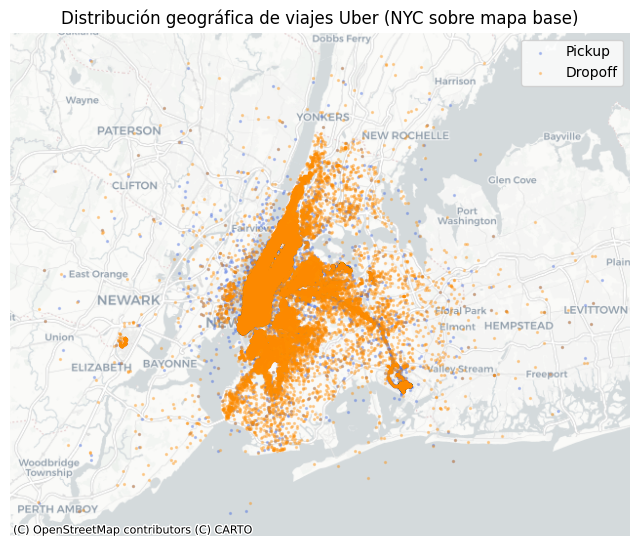
\includegraphics[width=0.70\textwidth,height=0.30\textheight,keepaspectratio]{../figures/2.png}
		\caption{Distribución geográfica de los puntos de origen (\textit{pickup}) y destino (\textit{dropoff}) de los viajes Uber en la ciudad de Nueva York.}
		\label{fig:uber_mapa_geografico}
	\end{figure}

	El mapa permite verificar visualmente que, tras la aplicación de los filtros geográficos, el conjunto de datos mantiene una cobertura espacial coherente con los límites definidos para el estudio.

	Para caracterizar la concentración espacial de los viajes y distinguir las zonas de mayor actividad, se generó un mapa de densidad mediante celdas hexagonales (\textit{Hexbin}) sobre la proyección geográfica de Nueva York. Este tipo de visualización permite representar la frecuencia de puntos de recogida (\textit{pickups}) en una escala logarítmica, lo que facilita la identificación de patrones urbanos sin perder detalle en áreas con alta densidad.

	Como se aprecia en la \figuraref{fig:uber_hexbin_pickups}, los resultados muestran una marcada concentración de puntos de recogida en Manhattan, especialmente en el sector sur y medio. También se observan focos de actividad en Brooklyn y Queens, así como en zonas de acceso hacia el aeropuerto JFK.

	\begin{figure}[!htbp]
		\centering
		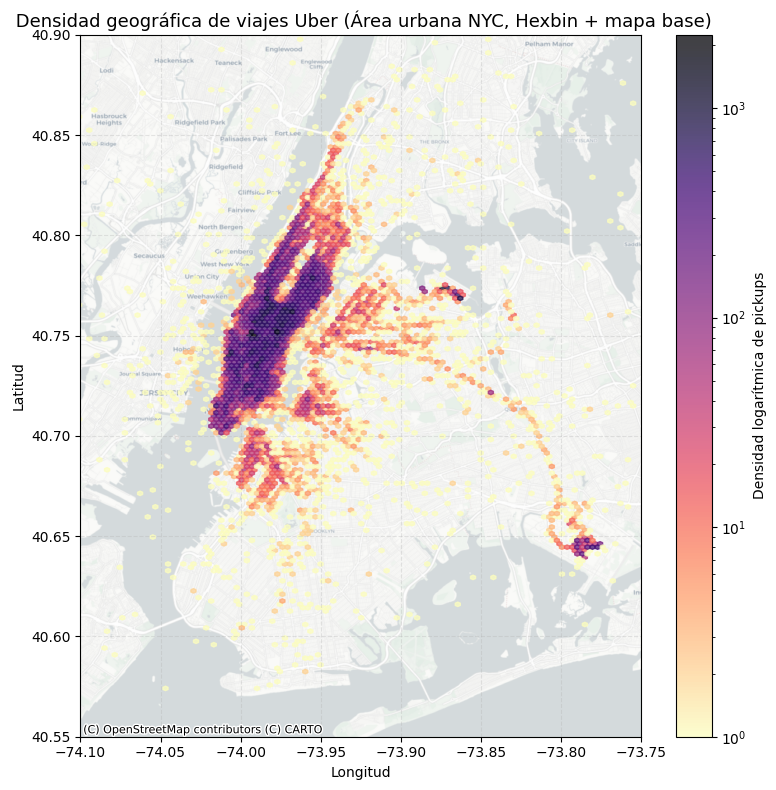
\includegraphics[width=0.66\textwidth,height=0.30\textheight,keepaspectratio]{../figures/4.png}
		\caption{Mapa de densidad de puntos de recogida (\textit{pickups}) de viajes Uber en el área urbana de Nueva York, utilizando celdas hexagonales (\textit{Hexbin}) y escala logarítmica.}
		\label{fig:uber_hexbin_pickups}
	\end{figure}

	Esta representación espacial permite visualizar con mayor claridad la concentración de observaciones en zonas de alta densidad. El uso de celdas \textit{Hexbin} mitiga el solapamiento de puntos y facilita la lectura de patrones espaciales.

	De forma complementaria, se incorporó un mapa de calor de densidad sobre mapa base para representar la intensidad espacial de los puntos de recogida. La \figuraref{fig:uber_kde_pickups} permite observar con mayor claridad el núcleo principal de viajes en Manhattan y su extensión hacia zonas cercanas de Brooklyn y Queens.

	\begin{figure}[!htbp]
		\centering
		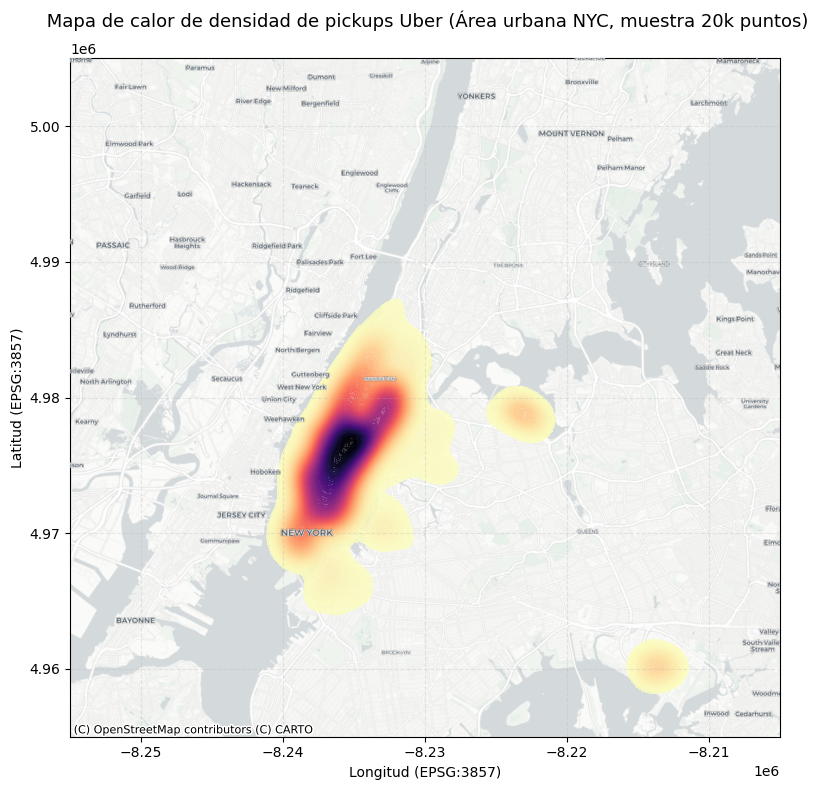
\includegraphics[width=0.68\textwidth,height=0.32\textheight,keepaspectratio]{../figures/6.png}
		\caption{Mapa de calor de densidad de puntos de recogida (\textit{pickups}) de viajes Uber sobre mapa base de Nueva York.}
		\label{fig:uber_kde_pickups}
	\end{figure}

	Con el fin de cuantificar las relaciones entre las variables principales del conjunto de datos, se calculó la matriz de correlaciones de Pearson. Este análisis permite identificar asociaciones lineales y verificar la coherencia entre las medidas geográficas, la distancia recorrida y el valor de la tarifa.

	Los resultados se presentan en la \figuraref{fig:uber_correlaciones}, donde se observa una correlación positiva alta (\(r = 0.86\)) entre \texttt{fare\_amount} y \texttt{distance\_km}. Este resultado respalda el uso de la distancia como predictor principal de la tarifa. Asimismo, se evidencian correlaciones moderadas entre las coordenadas de origen y destino, asociadas con la estructura espacial de los registros.

	\begin{figure}[!htbp]
		\centering
		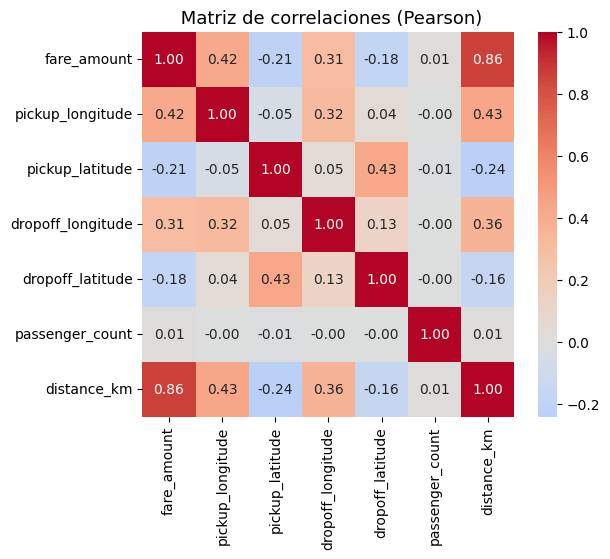
\includegraphics[width=0.66\textwidth,height=0.28\textheight,keepaspectratio]{../figures/7.png}
		\caption{Matriz de correlaciones de Pearson entre las variables principales del dataset de viajes Uber. Se destaca la fuerte correlación positiva entre \texttt{fare\_amount} y \texttt{distance\_km}.}
		\label{fig:uber_correlaciones}
	\end{figure}

	En conjunto, estos resultados sustentan la selección de \texttt{distance\_km} como variable predictora principal en los modelos de regresión y aprendizaje automático aplicados en las etapas posteriores.

	Con el objetivo de complementar el análisis de correlaciones lineales, se aplicó el coeficiente de Spearman, que permite evaluar relaciones monótonas entre variables sin asumir linealidad. Este enfoque resulta especialmente útil en contextos donde las variables pueden presentar distribuciones no normales o efectos de saturación, como ocurre en los datos de transporte urbano.

	La \figuraref{fig:uber_correlaciones_spearman} muestra la matriz de correlaciones obtenida mediante este método. Los resultados indican una relación monótona positiva alta (\(\rho = 0.85\)) entre \texttt{fare\_amount} y \texttt{distance\_km}, en concordancia con los hallazgos del análisis de Pearson (\figuraref{fig:uber_correlaciones}). Asimismo, se observan asociaciones moderadas entre las coordenadas geográficas de origen y destino.

	\begin{figure}[!htbp]
		\centering
		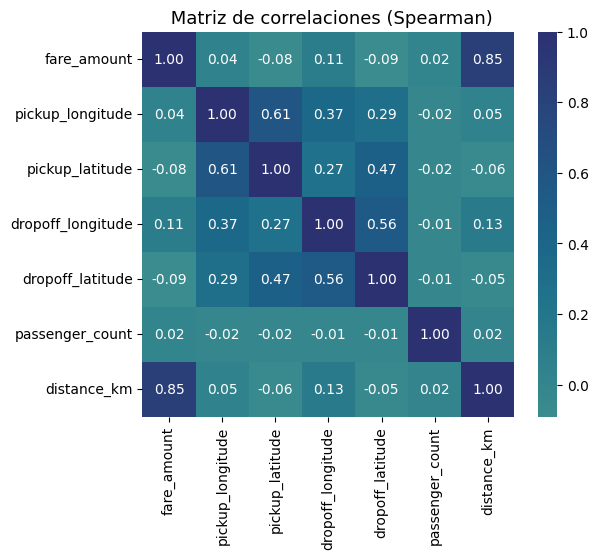
\includegraphics[width=0.66\textwidth,height=0.28\textheight,keepaspectratio]{../figures/8.png}
		\caption{Matriz de correlaciones de Spearman entre las variables principales del dataset de viajes Uber. Se observa una fuerte correlación monótona positiva entre \texttt{fare\_amount} y \texttt{distance\_km}.}
		\label{fig:uber_correlaciones_spearman}
	\end{figure}

	La comparación entre ambas métricas muestra que la relación entre tarifa y distancia se mantiene alta bajo criterios de asociación lineal y monótona. Este resultado respalda la selección de \texttt{distance\_km} como predictor principal en los modelos que se presentan en la siguiente sección.

	\subsection{Partición de datos}

	Para evaluar la capacidad de generalización de los modelos, el dataset final de 179\,855 observaciones se dividió en dos subconjuntos mediante \texttt{train\_test\_split} de \texttt{scikit-learn}: 80\,\% para entrenamiento y 20\,\% para prueba. El número de documento del estudiante se utilizó como semilla aleatoria (\texttt{random\_state = 1073247388}) para asegurar la reproducibilidad de la partición. El conjunto de entrenamiento se empleó para ajustar los modelos y realizar validación cruzada cuando correspondía, mientras que el conjunto de prueba se reservó para la evaluación final.

	El \cuadroref{tab:particion_dataset} presenta el resumen de esta partición, indicando el tamaño final de cada subconjunto.

	\begin{table}[!htbp]
		\centering
		\caption{Partición del conjunto de datos para entrenamiento y prueba.}
		\label{tab:particion_dataset}
		\begin{adjustbox}{max width=0.95\textwidth,center}
			\begin{tabular}{lc}
				\hline
				\textbf{Descripción} & \textbf{Valor} \\
				\hline
				Tamaño total del dataset & 179{,}855 observaciones \\
				Proporción de entrenamiento & 80\% (143{,}884 observaciones) \\
				Proporción de prueba & 20\% (35{,}971 observaciones) \\
				Random state utilizado & 1073247388 \\
				\hline
			\end{tabular}
		\end{adjustbox}
	\end{table}

	Esta división constituye la base de comparación final para todos los modelos. En los modelos de ensamble y redes neuronales se utilizó un submuestreo reproducible de 90\,000 observaciones del conjunto de entrenamiento para la búsqueda de hiperparámetros y selección de arquitectura, manteniendo el mismo \texttt{random\_state}; posteriormente, los modelos seleccionados se reentrenaron y evaluaron sobre el conjunto de prueba oficial.


	\subsection{Modelado predictivo}
	El modelado predictivo tuvo como variable objetivo \texttt{fare\_amount}. Además de la distancia recorrida (\texttt{distance\_km}), se incorporaron cantidad de pasajeros, hora, día de la semana, mes, año del viaje y coordenadas geográficas de origen y destino. La distancia se mantiene como variable principal, mientras que las variables adicionales permiten capturar patrones temporales y espaciales no representados por una especificación univariada. Se implementaron cinco enfoques de modelado supervisado:
	\begin{enumerate}[label=\alph*)]
		\item \textbf{Regresión lineal (MCO):} modelo base que estima efectos promedio bajo una especificación lineal ampliada, útil para interpretación económica.
		\item \textbf{Regresión LASSO:} versión regularizada del modelo lineal que incorpora penalización $L_1$ para prevenir sobreajuste y controlar la magnitud de los coeficientes.
		\item \textbf{Random Forest:} ensamble de árboles de decisión utilizado para evaluar si una especificación no lineal mejora la predicción frente a los modelos lineales.
		\item \textbf{Gradient Boosting:} modelo secuencial que ajusta sucesivos árboles a los errores del modelo anterior, incorporando hiperparámetros como número de estimadores, profundidad y tasa de aprendizaje.
		\item \textbf{Redes neuronales densas:} cuatro arquitecturas del tipo \textit{feedforward} con diferente número de capas ocultas, activación ReLU y optimizador Adam.
	\end{enumerate}

	Para los modelos Random Forest, Gradient Boosting y redes neuronales se trabajó con submuestras de 90\,000 observaciones del conjunto de entrenamiento durante la etapa de búsqueda de hiperparámetros o selección de arquitectura, con el fin de equilibrar robustez, tiempo de entrenamiento y reproducibilidad local. La evaluación final de todos los modelos se realizó sobre el mismo conjunto de prueba definido en el Punto 3.

	\subsection{Métricas de evaluación}
	El desempeño de los modelos se midió principalmente mediante métricas de error calculadas sobre datos de prueba:
	\begin{itemize}
		\item \textbf{RMSE (Root Mean Squared Error):} raíz del error cuadrático medio; penaliza errores grandes y refleja la precisión general del modelo.
		\[
		RMSE = \sqrt{\frac{1}{n}\sum_{i=1}^{n}(\hat{y}_i - y_i)^2}
		\]
		\item \textbf{MAE (Mean Absolute Error):} promedio de los errores absolutos; es menos sensible a valores extremos.
		\[
		MAE = \frac{1}{n}\sum_{i=1}^{n}|\hat{y}_i - y_i|
		\]
		\item \textbf{Coeficiente de determinación ($R^2$):} proporción de la variabilidad explicada por el modelo respecto a la variabilidad total, reportada principalmente para los modelos lineales.
	\end{itemize}
	La comparación final entre modelos se realizó con RMSE y MAE, priorizando el desempeño fuera de muestra. Un menor valor de estas métricas indica menor error promedio de predicción.

	\subsection{Reproducibilidad}
	Todo el proceso fue desarrollado en un notebook de Jupyter con \texttt{Python 3.x}, utilizando las librerías \texttt{pandas}, \texttt{numpy}, \texttt{matplotlib}, \texttt{seaborn}, \texttt{scikit-learn} y \texttt{tensorflow/keras}. Para facilitar la reproducción, el notebook carga el archivo \texttt{data/uber.csv} de forma local, utiliza \texttt{random\_state = 1073247388} y documenta las etapas de lectura, limpieza, visualización, entrenamiento y evaluación de modelos.

	\section{Resultados}

	\subsection{Relación entre variables continuas (Tarifa vs. Distancia)}

	Tras el análisis individual de las variables \texttt{fare\_amount} y \texttt{distance\_km}, resulta pertinente examinar su relación conjunta con el fin de identificar patrones de dependencia entre la distancia recorrida y el valor de la tarifa. La \figuraref{fig:relacion_fare_distance} presenta la nube de puntos correspondiente al dataset filtrado, junto con la línea de tendencia ajustada mediante un modelo lineal simple.

	Como puede observarse, existe una marcada relación positiva entre ambas variables: a medida que la distancia aumenta, la tarifa también tiende a incrementarse de forma aproximadamente proporcional. Esta tendencia es consistente con los resultados de correlación obtenidos previamente en las \figuraref{fig:uber_correlaciones} y \figuraref{fig:uber_correlaciones_spearman}, donde se observó una asociación positiva alta entre ambas magnitudes.

	El patrón lineal visible en el gráfico es compatible con una estructura de precios en la que la distancia recorrida cumple un papel central. Las desviaciones respecto de la tendencia pueden estar asociadas a factores no observados en el dataset, como el tiempo de espera, el tráfico, tarifas mínimas o mecanismos de demanda dinámica.

	\begin{figure}[!htbp]
		\centering
		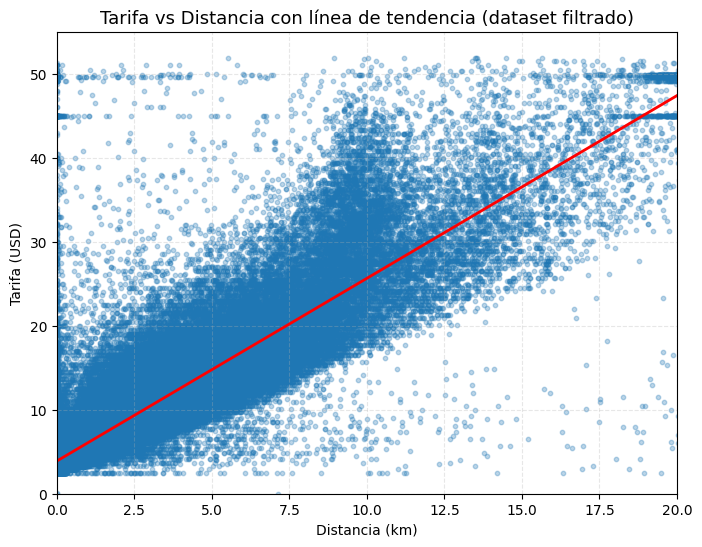
\includegraphics[width=0.66\textwidth,height=0.30\textheight,keepaspectratio]{../figures/13.png}
		\caption{Relación entre la distancia recorrida (\texttt{distance\_km}) y la tarifa del viaje (\texttt{fare\_amount}) en el dataset filtrado. Se observa una asociación positiva con una tendencia aproximadamente lineal.}
		\label{fig:relacion_fare_distance}
	\end{figure}

	\subsection{Resultados de los modelos lineales}

	El primer modelo estimado corresponde a una regresión lineal ordinaria (OLS) sobre el conjunto ampliado de predictores. Este enfoque se utiliza como referencia interpretable y como base de comparación frente a modelos más flexibles.

	Como se muestra en el \cuadroref{tab:ols_resultados}, el modelo alcanza un coeficiente de determinación $R^2 = 0.706$, lo que indica que aproximadamente el 70.6\% de la variabilidad de la tarifa queda explicada por esta especificación. El coeficiente asociado a \texttt{distance\_km} es positivo ($\beta = 2.0057$) y estadísticamente significativo ($p < 0.001$), por lo que, manteniendo constantes las demás variables incluidas, cada kilómetro adicional se asocia con un aumento promedio cercano a 2.01~USD en la tarifa.

	Las variables temporales y geográficas también resultan estadísticamente significativas, aunque su interpretación debe ser cautelosa por la escala de las coordenadas y la posible colinealidad entre variables espaciales. Por ello, OLS se utiliza como referencia interpretable y no como especificación causal.

	\begin{table}[!htbp]
		\centering
		\caption{Resultados del modelo de regresión lineal (OLS) con conjunto ampliado de predictores.}
		\label{tab:ols_resultados}
		\begin{adjustbox}{max width=0.95\textwidth,center}
			\begin{tabular}{lcc}
				\hline
				\textbf{Variable} & \textbf{Coef.} & \textbf{P$>|t|$} \\
				\hline
				Constante & 117.4767 & 0.000 \\
				\texttt{distance\_km} & 2.0057 & 0.000 \\
				\texttt{passenger\_count} & 0.0376 & 0.000 \\
				\texttt{pickup\_hour} & 0.0115 & 0.000 \\
				\texttt{pickup\_dayofweek} & -0.0343 & 0.000 \\
				\texttt{pickup\_month} & 0.0571 & 0.000 \\
				\texttt{pickup\_year} & 0.3865 & 0.000 \\
				\texttt{pickup\_longitude} & 2.3192 & 0.000 \\
				\texttt{pickup\_latitude} & 2.1465 & 0.000 \\
				\texttt{dropoff\_longitude} & 3.7267 & 0.000 \\
				\texttt{dropoff\_latitude} & -13.0475 & 0.000 \\
				\hline
				\multicolumn{3}{l}{\textbf{Indicadores del modelo:}} \\
				\hline
				\textit{R$^2$} & \multicolumn{2}{c}{0.706} \\
				\textit{AIC} & \multicolumn{2}{c}{6.558e+05} \\
				\textit{BIC} & \multicolumn{2}{c}{6.559e+05} \\
				\textit{No. de observaciones} & \multicolumn{2}{c}{143{,}884} \\
				\hline
			\end{tabular}
		\end{adjustbox}
	\end{table}

	A fin de complementar el modelo OLS, se aplicó una regresión LASSO (Least Absolute Shrinkage and Selection Operator), previa estandarización de las variables explicativas. En esta especificación multivariable, LASSO permite evaluar si la penalización $L_1$ elimina predictores o conserva el conjunto de variables propuesto.

	Los resultados del modelo ajustado se presentan en el \cuadroref{tab:lasso_resultados}. El parámetro de regularización óptimo obtenido mediante validación cruzada fue $\lambda = 0.0001$, lo que indica una penalización muy baja. Ninguna variable fue reducida exactamente a cero. El coeficiente estandarizado de mayor magnitud corresponde a \texttt{distance\_km}, seguido por \texttt{pickup\_year} y algunas variables geográficas.

	El coeficiente de LASSO no debe compararse directamente con los coeficientes de OLS, dado que el modelo regularizado se estimó sobre variables escaladas. En términos predictivos, su desempeño final es prácticamente idéntico al del modelo lineal base, por lo que funciona como referencia regularizada antes de pasar a los modelos no lineales.

	\begin{table}[!htbp]
		\centering
		\caption{Parámetros del modelo LASSO ajustado con variables estandarizadas.}
		\label{tab:lasso_resultados}
		\begin{tabular}{lc}
			\hline
			\textbf{Parámetro} & \textbf{Valor} \\
			\hline
			Alpha óptimo ($\lambda$) & 0.0001 \\
			Coeficiente estandarizado de \texttt{distance\_km} & 3.5583 \\
			Coeficiente estandarizado de \texttt{pickup\_year} & 0.7175 \\
			Variables eliminadas & 0 \\
			Intercepto & 9.0575 \\
			\hline
		\end{tabular}
	\end{table}


	\subsection{Resultados de los modelos de ensamble}

	Para capturar posibles relaciones no lineales entre las variables disponibles y la tarifa, se estimaron modelos de tipo \textit{ensemble}. El primero fue \textit{Random Forest}, que combina múltiples árboles de decisión y promedia sus predicciones.

	La búsqueda de hiperparámetros se realizó con una submuestra de 90{,}000 observaciones del conjunto de entrenamiento oficial. Se exploraron 16 combinaciones mediante validación cruzada de tres particiones. Los mejores valores se resumen en el \cuadroref{tab:rf_resultados}: árboles sin profundidad máxima predefinida, mínimo de 2 observaciones por división, selección de variables \texttt{sqrt} y 500 estimadores.

	Tras seleccionar los hiperparámetros, el modelo se reentrenó con todo el conjunto de entrenamiento oficial y se evaluó sobre el test del Punto 3. Alcanzó un RMSE de 1.9907 y un MAE de 1.3334. La importancia de variables ubica a \texttt{distance\_km} como predictor dominante, seguido por coordenadas geográficas y variables temporales de menor peso relativo.

	\begin{table}[!htbp]
		\centering
		\caption{Resultados del modelo \textit{Random Forest} aplicado a la predicción de \texttt{fare\_amount}.}
		\label{tab:rf_resultados}
		\begin{adjustbox}{max width=0.95\textwidth,center}
			\begin{tabular}{lc}
				\hline
				\textbf{Descripción} & \textbf{Valor} \\
				\hline
				Submuestra para búsqueda de hiperparámetros & 90{,}000 observaciones del entrenamiento \\
				Conjunto de entrenamiento para tuning & 72{,}000 registros (80\%) \\
				Conjunto de validación para tuning & 18{,}000 registros (20\%) \\
				Base de evaluación final & Test oficial del Punto 3 \\
				Número total de combinaciones evaluadas & 16 \\
				\hline
				\multicolumn{2}{l}{\textbf{Mejores hiperparámetros encontrados:}} \\
				\hline
				\texttt{max\_depth} & Sin límite \\
				\texttt{max\_features} & \texttt{sqrt} \\
				\texttt{min\_samples\_split} & 2 \\
				\texttt{n\_estimators} & 500 \\
				\hline
				\multicolumn{2}{l}{\textbf{Evaluación del modelo:}} \\
				\hline
				RMSE validación & 2.0506 \\
				MAE validación & 1.3795 \\
				RMSE test oficial & 1.9907 \\
				MAE test oficial & 1.3334 \\
				\hline
			\end{tabular}
		\end{adjustbox}
	\end{table}

	La \figuraref{fig:random_forest_prediccion} muestra la relación entre valores reales y predichos. La concentración alrededor de la diagonal indica que el modelo reproduce el patrón general de las tarifas, aunque persiste dispersión en algunos rangos.

	\begin{figure}[!htbp]
		\centering
		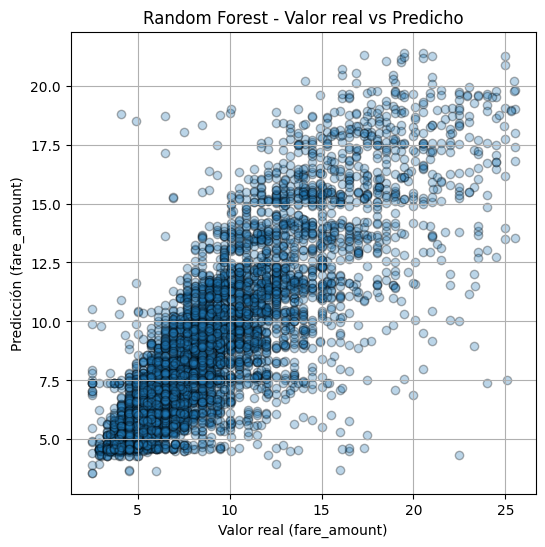
\includegraphics[width=0.58\textwidth,height=0.30\textheight,keepaspectratio]{../figures/16.png}
		\caption{Relación entre valores reales y predichos del modelo \textit{Random Forest} para la variable \texttt{fare\_amount}. Se observa una tendencia positiva y una dispersión moderada alrededor de la línea de referencia.}
		\label{fig:random_forest_prediccion}
	\end{figure}

	El segundo modelo de ensamble fue \textit{Gradient Boosting}, que construye árboles de forma secuencial para corregir errores residuales del modelo anterior.

	La búsqueda de hiperparámetros se realizó sobre una submuestra de 90{,}000 observaciones del conjunto de entrenamiento oficial. Se evaluaron 24 combinaciones mediante validación cruzada de tres particiones. A diferencia de \textit{Random Forest}, \textit{Gradient Boosting} construye árboles de forma iterativa, corrigiendo errores residuales del ensamble previo.

	Los mejores resultados se alcanzaron con una tasa de aprendizaje de 0.1, profundidad máxima de 5 niveles, 500 estimadores y \texttt{subsample = 0.8}. Tras reentrenar el modelo con todo el conjunto de entrenamiento oficial, obtuvo un RMSE de 1.9429 y un MAE de 1.2753 sobre el test del Punto 3. Al igual que en \textit{Random Forest}, la variable \texttt{distance\_km} concentra la mayor importancia relativa.

	\begin{table}[!htbp]
		\centering
		\caption{Resultados del modelo \textit{Gradient Boosting} aplicado a la predicción de \texttt{fare\_amount}.}
		\label{tab:gb_resultados}
		\begin{adjustbox}{max width=0.95\textwidth,center}
			\begin{tabular}{lc}
				\hline
				\textbf{Descripción} & \textbf{Valor} \\
				\hline
				Submuestra para búsqueda de hiperparámetros & 90{,}000 observaciones del entrenamiento \\
				Conjunto de entrenamiento para tuning & 72{,}000 registros (80\%) \\
				Conjunto de validación para tuning & 18{,}000 registros (20\%) \\
				Base de evaluación final & Test oficial del Punto 3 \\
				Número total de combinaciones evaluadas & 24 \\
				\hline
				\multicolumn{2}{l}{\textbf{Mejores hiperparámetros encontrados:}} \\
				\hline
				\texttt{learning\_rate} & 0.1 \\
				\texttt{max\_depth} & 5 \\
				\texttt{n\_estimators} & 500 \\
				\texttt{subsample} & 0.8 \\
				\hline
				\multicolumn{2}{l}{\textbf{Evaluación del modelo:}} \\
				\hline
				RMSE validación & 1.9990 \\
				MAE validación & 1.3015 \\
				RMSE test oficial & 1.9429 \\
				MAE test oficial & 1.2753 \\
				\hline
			\end{tabular}
		\end{adjustbox}
	\end{table}

	La \figuraref{fig:gradient_boosting_prediccion} muestra una alineación clara entre valores reales y predichos, con dispersión mayor en tarifas altas. Este patrón es consistente con una mejora predictiva respecto de los modelos lineales.

	\begin{figure}[!htbp]
		\centering
		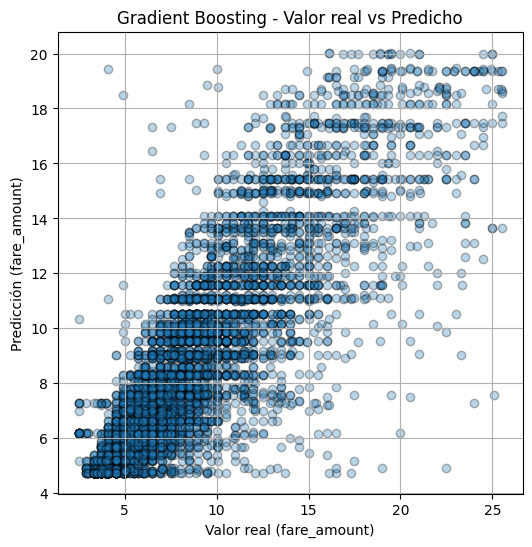
\includegraphics[width=0.58\textwidth,height=0.30\textheight,keepaspectratio]{../figures/17.png}
		\caption{Relación entre valores reales y predichos del modelo \textit{Gradient Boosting} para la variable \texttt{fare\_amount}. Se observa un ajuste consistente con dispersión moderada alrededor de la línea de referencia.}
		\label{fig:gradient_boosting_prediccion}
	\end{figure}

	\subsection{Resultados de las redes neuronales}

	Como complemento a los modelos basados en árboles, se implementaron cuatro arquitecturas de redes neuronales densas. La selección se realizó sobre una submuestra de 90{,}000 observaciones del conjunto de entrenamiento, usando activación ReLU, optimización Adam y parada temprana. La mejor arquitectura se reentrenó con el conjunto de entrenamiento oficial y se evaluó sobre el test del Punto 3.

	El desempeño de cada red se evaluó con RMSE y MAE, como se resume en el \cuadroref{tab:nn_resultados}. En validación, la arquitectura con cuatro capas ocultas presentó el menor RMSE. En el test oficial obtuvo un RMSE de 1.9149 y un MAE de 1.2327, convirtiéndose en el modelo con mejor desempeño global del ejercicio.

	\begin{table}[!htbp]
		\centering
		\caption{Resultados de validación de las arquitecturas de red neuronal durante la etapa de selección.}
		\label{tab:nn_resultados}
		\begin{adjustbox}{max width=0.95\textwidth,center}
			\begin{tabular}{lccc}
				\hline
				\textbf{Arquitectura} & \textbf{RMSE validación} & \textbf{MAE validación} & \textbf{Épocas} \\
				\hline
				Modelo 1 (1 capa oculta, 32 neuronas) & 2.0648 & 1.3528 & 180 \\
				Modelo 2 (2 capas ocultas, 64--32 neuronas) & 2.0279 & 1.3109 & 52 \\
				Modelo 3 (3 capas ocultas, 128--64--32 neuronas) & 1.9959 & 1.2846 & 74 \\
				Modelo 4 (4 capas ocultas, 256--128--64--32 neuronas) & 1.9935 & 1.2827 & 67 \\
				\hline
			\end{tabular}
		\end{adjustbox}
	\end{table}

	\subsection{Comparación general de desempeño}

	Para responder al punto final de la consigna, se comparó el desempeño de todos los modelos sobre el mismo conjunto de prueba oficial definido en el Punto 3.

	\begin{table}[!htbp]
		\centering
		\caption{Desempeño final de los modelos sobre el conjunto de prueba oficial.}
		\label{tab:performance_final}
		\begin{adjustbox}{max width=0.95\textwidth,center}
			\begin{tabular}{lccc}
				\hline
				\textbf{Modelo} & \textbf{RMSE} & \textbf{MAE} & \textbf{Base de evaluación} \\
				\hline
				Red neuronal -- Modelo 4 & 1.9149 & 1.2327 & Test oficial Punto 3 \\
				\textit{Gradient Boosting} & 1.9429 & 1.2753 & Test oficial Punto 3 \\
				\textit{Random Forest} & 1.9907 & 1.3334 & Test oficial Punto 3 \\
				OLS & 2.3465 & 1.6362 & Test oficial Punto 3 \\
				LASSO & 2.3465 & 1.6362 & Test oficial Punto 3 \\
				\hline
			\end{tabular}
		\end{adjustbox}
	\end{table}

	La \figuraref{fig:performance_final_rmse} complementa la comparación tabular y ordena los modelos según RMSE. La red neuronal de cuatro capas ocultas alcanza el menor error, seguida de cerca por \textit{Gradient Boosting}. Los modelos lineales mejoran respecto de la especificación simple gracias al set ampliado de variables, aunque quedan por detrás de los enfoques no lineales.

	\begin{figure}[!htbp]
		\centering
		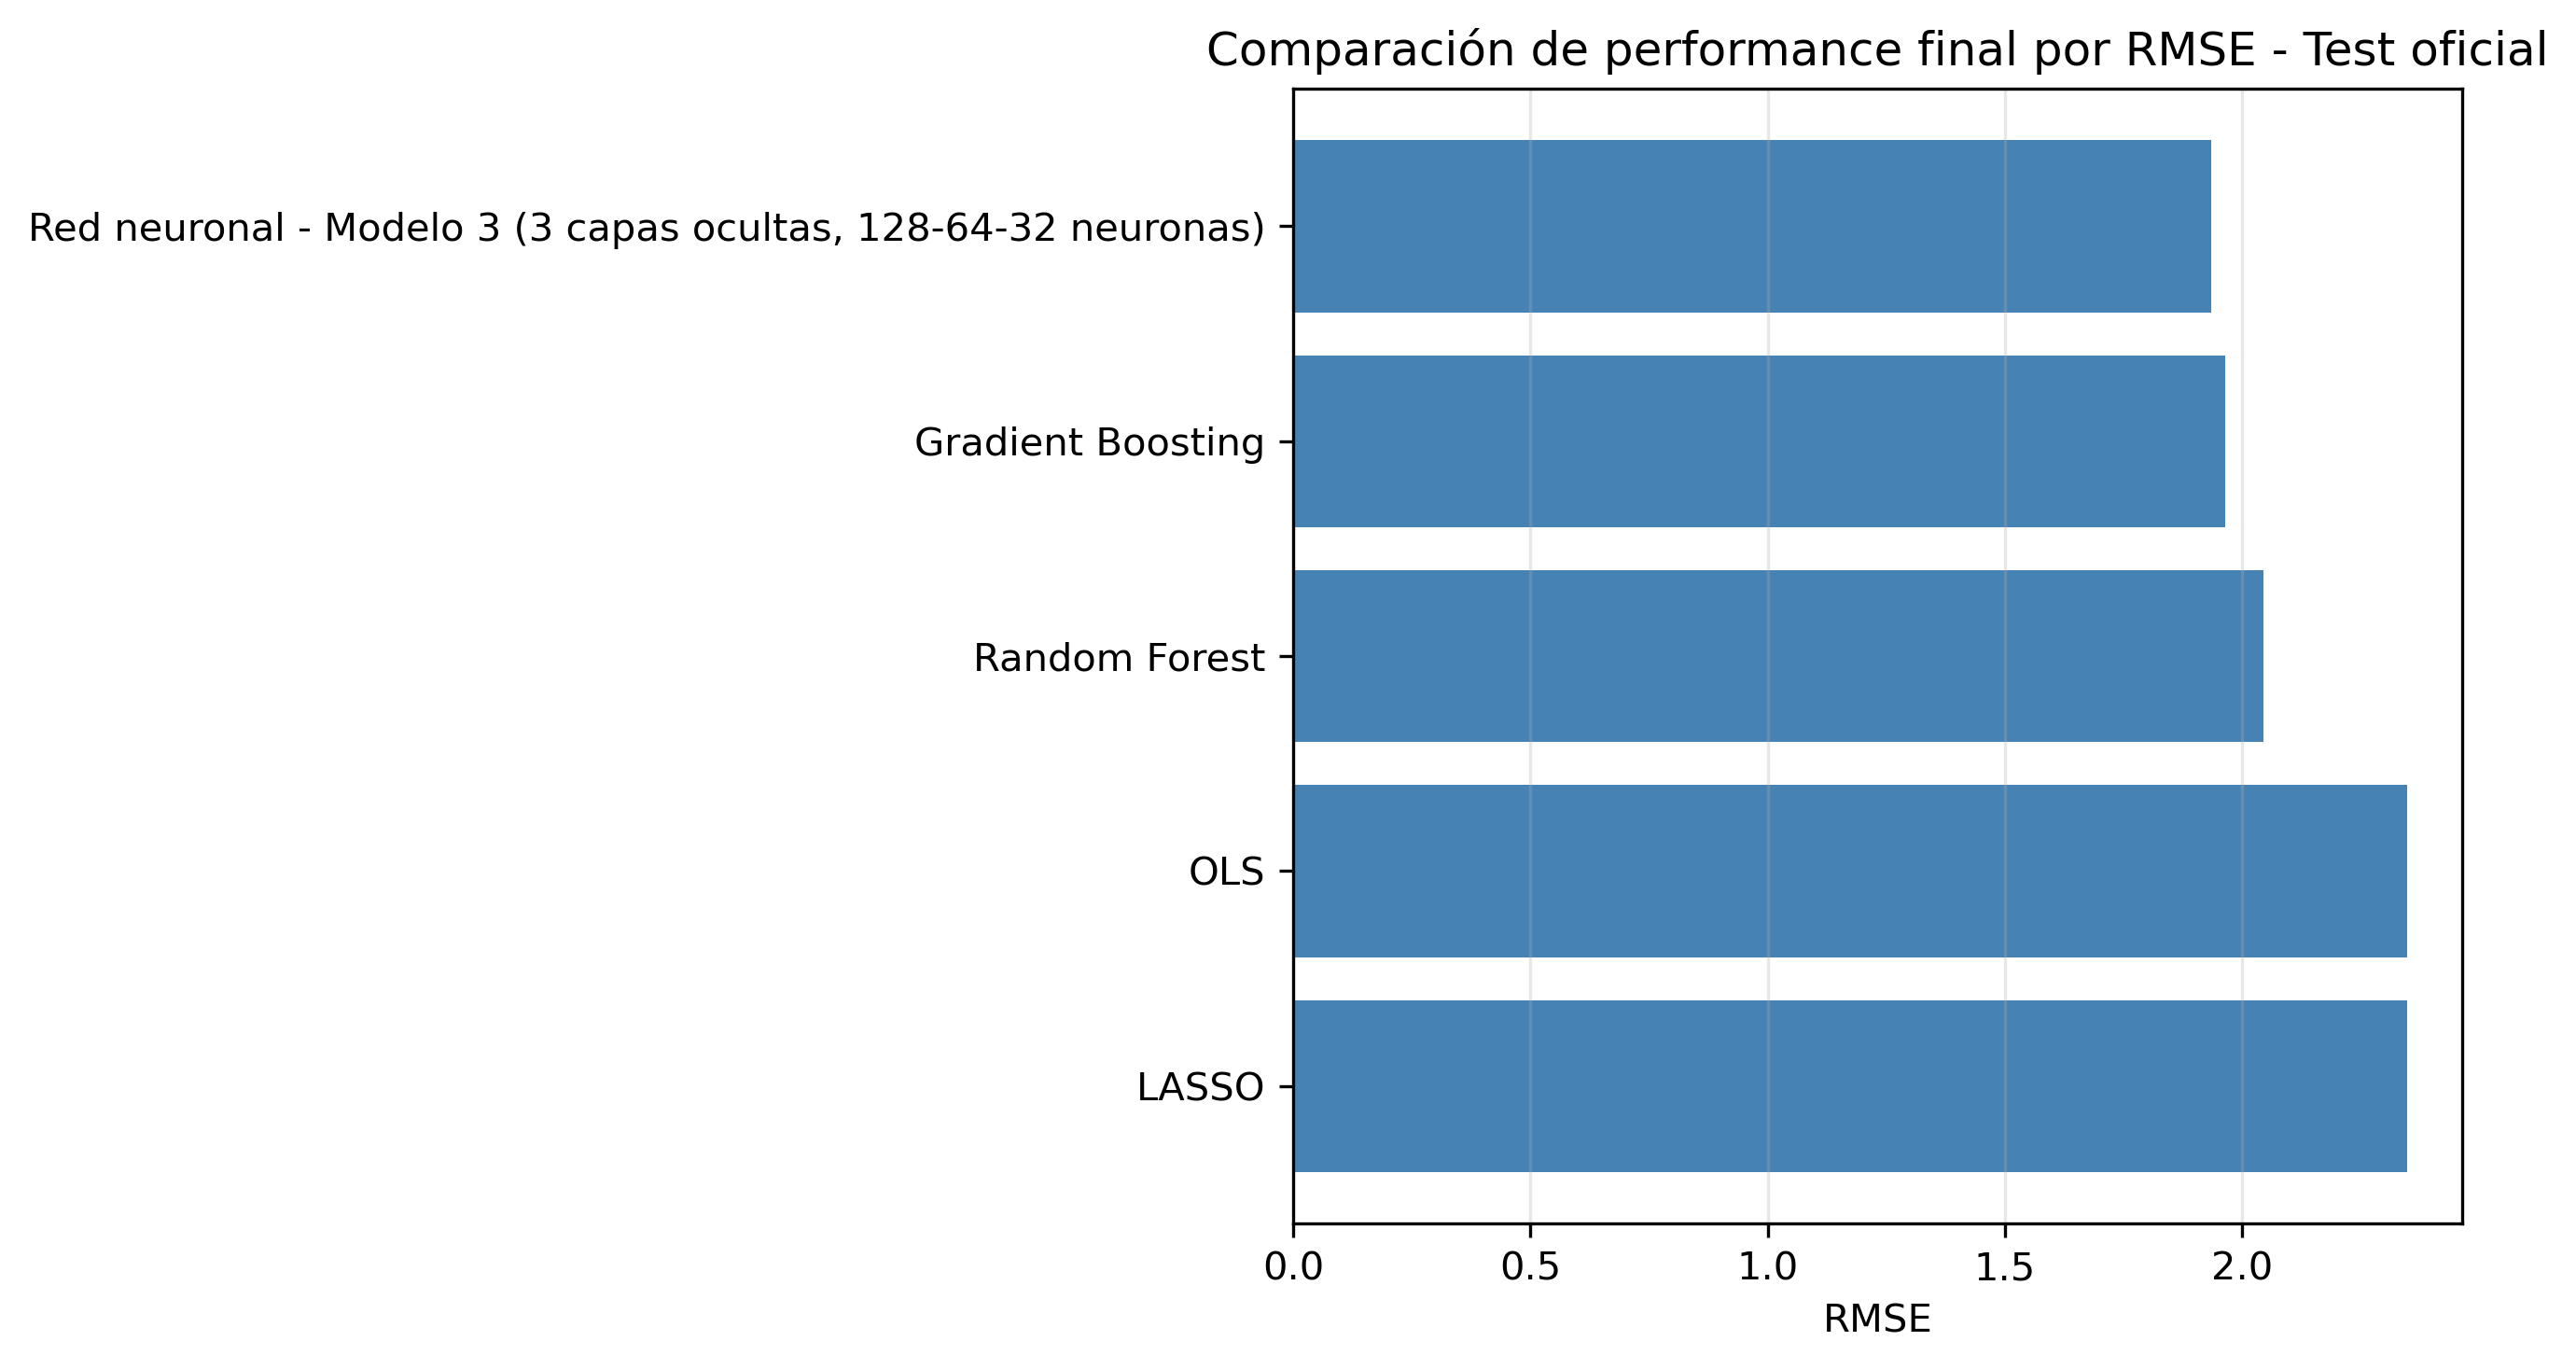
\includegraphics[width=0.78\textwidth,height=0.36\textheight,keepaspectratio]{../figures/19.png}
		\caption{Comparación del desempeño final por RMSE sobre el conjunto de prueba oficial.}
		\label{fig:performance_final_rmse}
	\end{figure}

	Adicionalmente, la \figuraref{fig:residuos_mejor_modelo} presenta un diagnóstico de residuos para la red neuronal de cuatro capas ocultas, identificada como el modelo con menor RMSE en la comparación final. La nube de puntos se concentra alrededor de cero, con mayor dispersión en algunos rangos de predicción.

	\begin{figure}[!htbp]
		\centering
		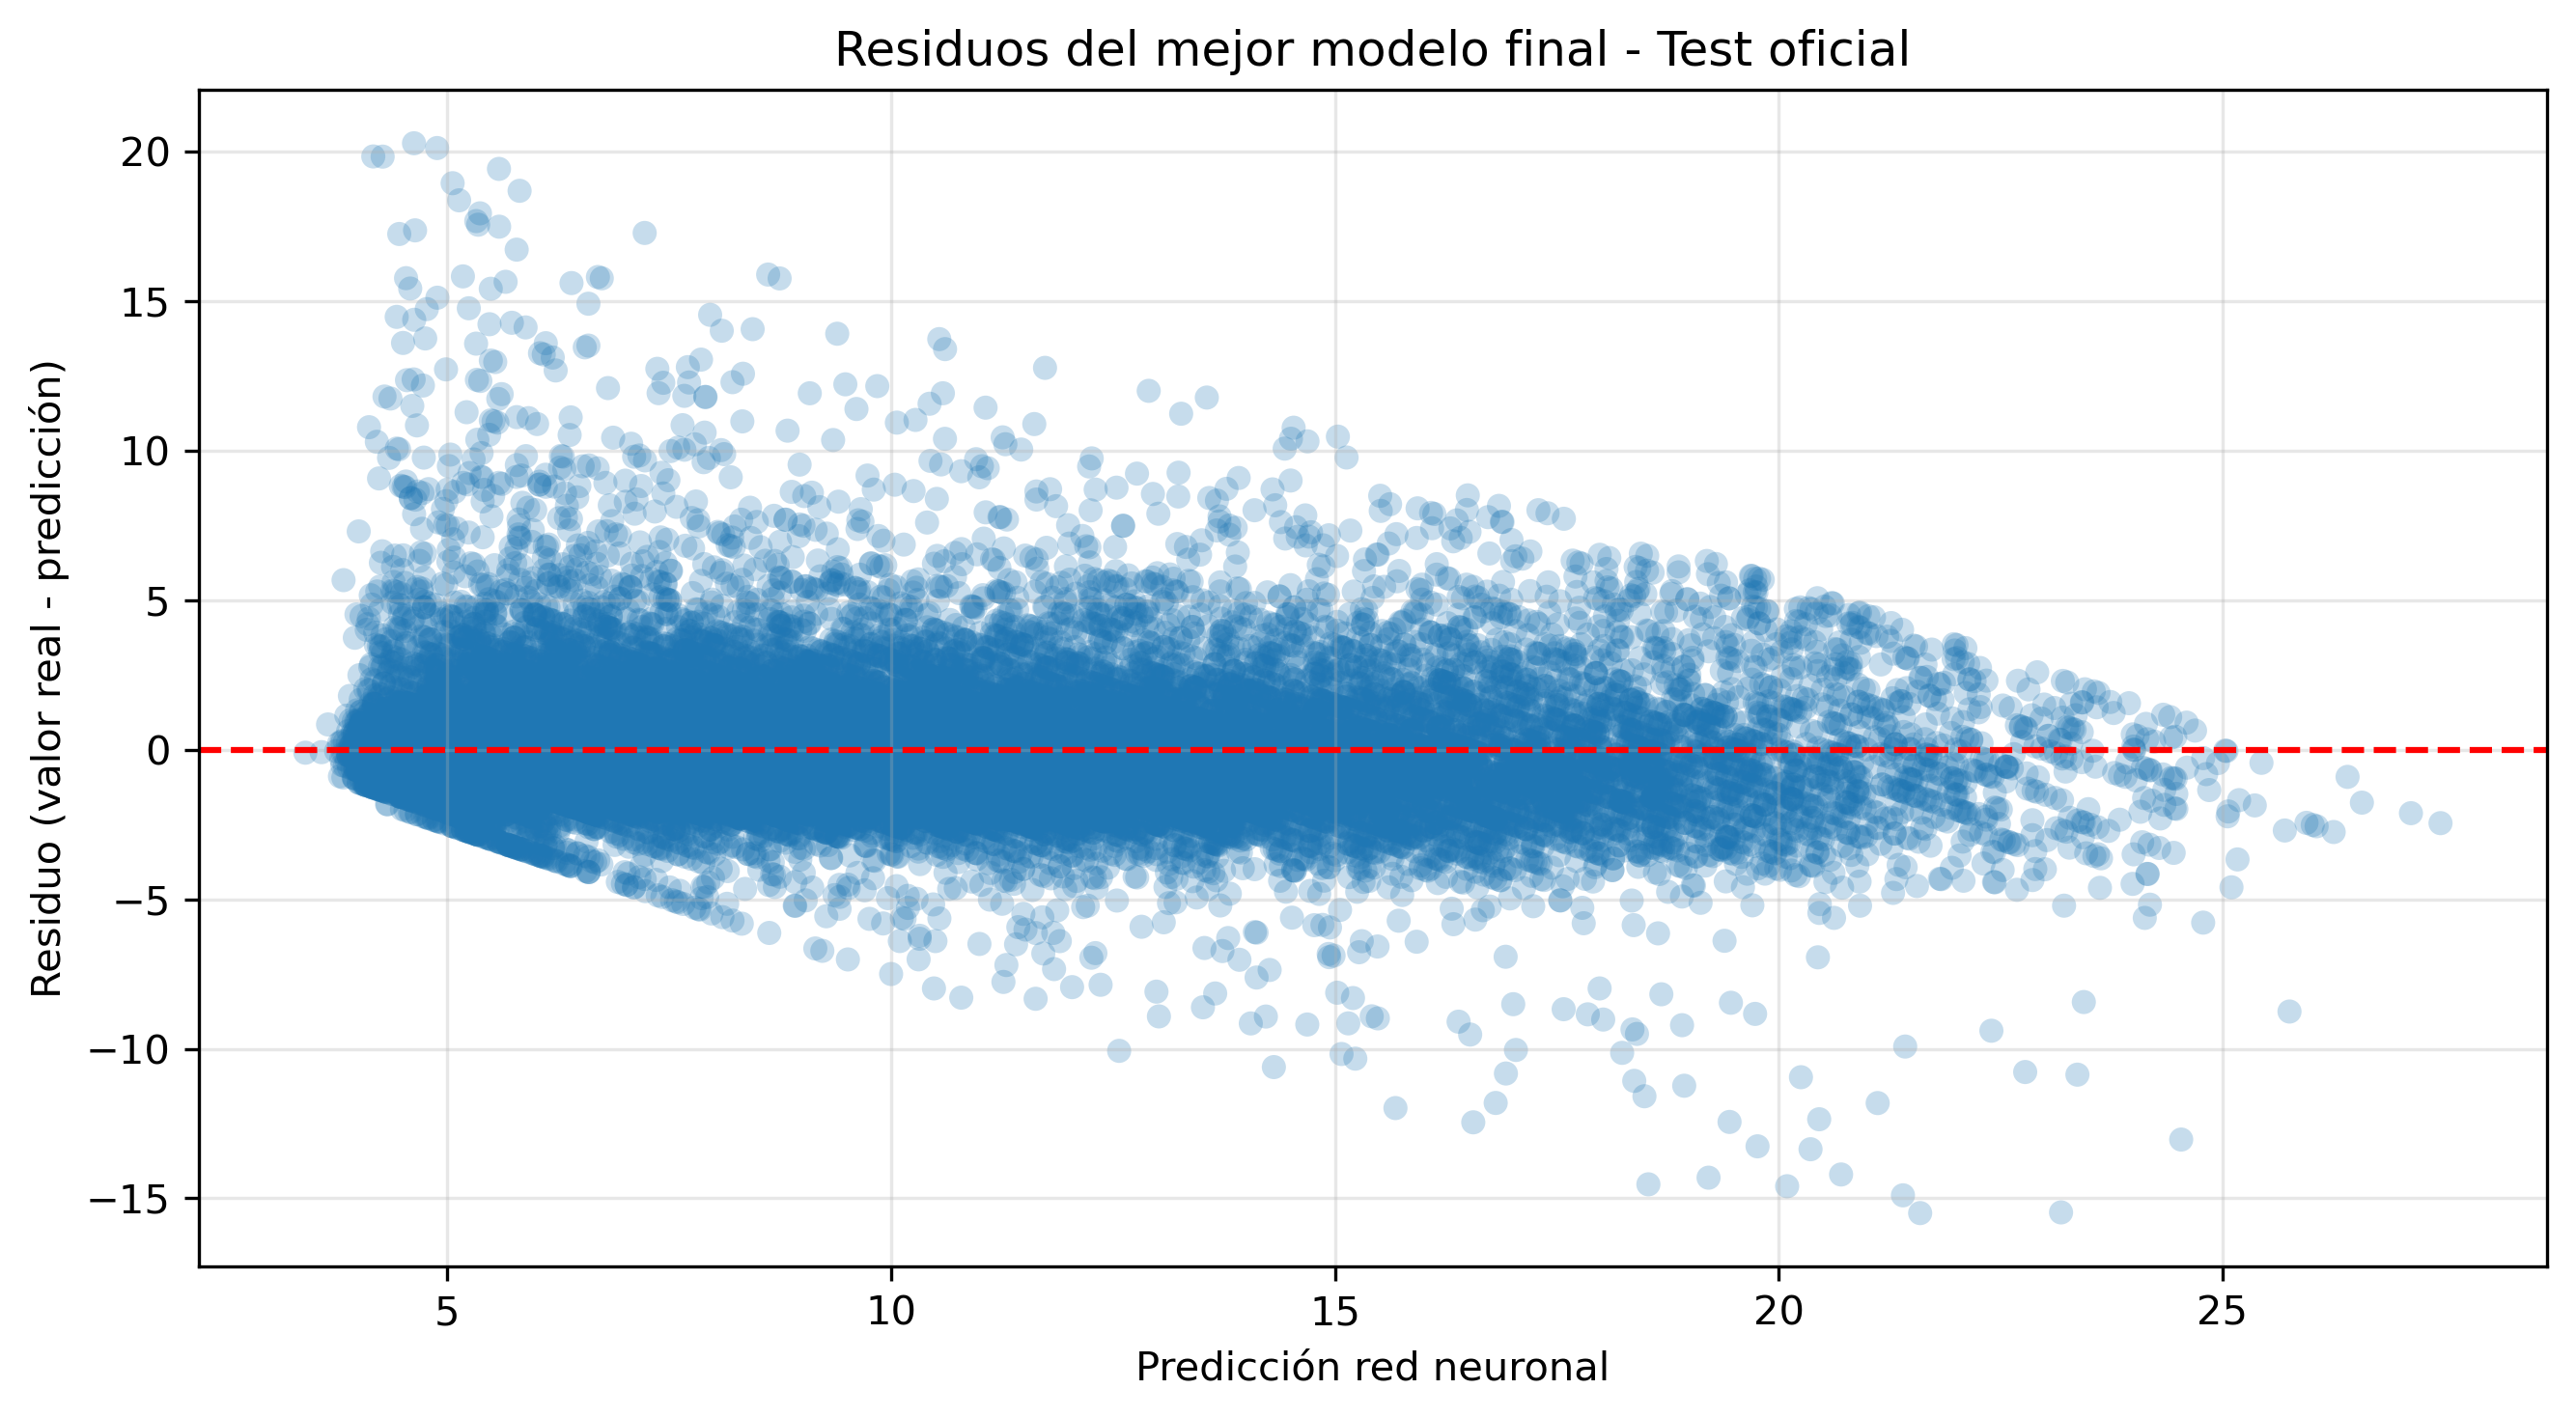
\includegraphics[width=0.74\textwidth,height=0.34\textheight,keepaspectratio]{../figures/20.png}
		\caption{Residuos del mejor modelo final, correspondiente a la red neuronal de cuatro capas ocultas, sobre el conjunto de prueba oficial.}
		\label{fig:residuos_mejor_modelo}
	\end{figure}

	En conjunto, los enfoques no lineales presentan una ventaja clara frente a los modelos lineales. La red neuronal de cuatro capas ocultas obtuvo el menor RMSE, seguida por \textit{Gradient Boosting} y \textit{Random Forest}. OLS y LASSO conservan valor como referencias interpretables y de bajo costo computacional.

	\section{Discusión}

	Los resultados muestran que la distancia recorrida es el principal predictor disponible de la tarifa, incluso después de incorporar variables temporales, cantidad de pasajeros y coordenadas geográficas. La relación positiva entre \texttt{distance\_km} y \texttt{fare\_amount} es consistente con una estructura de precios donde conviven un componente fijo y uno proporcional a la distancia. En ese sentido, el modelo lineal funciona como referencia interpretable de la tendencia general.

	La ampliación del set de predictores y el entrenamiento más amplio produjeron una mejora importante frente a la especificación basada únicamente en distancia. La red neuronal de cuatro capas ocultas obtuvo el menor error sobre el test oficial, mientras que \textit{Gradient Boosting} quedó muy cerca y ofrece una alternativa competitiva con mayor facilidad de interpretación mediante importancia de variables. Aun así, persisten errores asociados a factores no observados, especialmente en algunos rangos de tarifa.

	Estos resultados deben interpretarse dentro de los límites del dataset. Aunque se incorporaron variables temporales derivadas del momento del viaje, no se cuenta con información sobre duración real, tráfico, clima, demanda local, método de asignación del viaje o tarifas dinámicas, variables que podrían explicar parte de la dispersión restante. Además, el análisis se restringe a la ciudad de Nueva York, por lo que no conviene extrapolar los resultados directamente a otras ciudades sin una validación adicional.

	Desde una perspectiva de Inteligencia de Negocios, el ejercicio muestra que un flujo reproducible de limpieza, exploración y modelado permite construir una primera aproximación útil a la predicción de tarifas. Para una aplicación operativa, sería necesario enriquecer la base de datos con variables contextuales y validar la estabilidad del modelo en muestras más recientes.

	\section{Conclusiones}

	El trabajo permitió desarrollar un flujo completo de análisis predictivo aplicado a tarifas de viajes de Uber: lectura del dataset, depuración, cálculo de distancia mediante Haversine, análisis exploratorio, partición train/test, estimación de modelos y comparación final.

	La evidencia muestra que \texttt{distance\_km} es un predictor central de \texttt{fare\_amount}. El modelo OLS permitió interpretar esta relación de forma directa dentro de una especificación ampliada, mientras que LASSO ofreció una referencia regularizada sin modificar sustancialmente el desempeño del modelo lineal.

	En la comparación final sobre el test oficial, los modelos de aprendizaje automático obtuvieron una ventaja clara frente a los modelos lineales. La red neuronal de cuatro capas ocultas presentó el menor RMSE, seguida por \textit{Gradient Boosting} y \textit{Random Forest}. Este resultado sugiere que la predicción de tarifas mejora cuando la distancia se complementa con variables temporales y geográficas.

	La principal limitación del estudio es la ausencia de variables contextuales que pueden afectar la tarifa final, como duración efectiva del viaje, tráfico, clima, demanda o mecanismos de tarifa dinámica. Futuras extensiones deberían incorporar estas dimensiones, evaluar la estabilidad temporal del modelo y comparar su desempeño en otras ciudades o ventanas de tiempo.

	En síntesis, el análisis muestra que la ingeniería de variables y los modelos flexibles mejoran la predicción de tarifas frente a una especificación lineal simple. Al mismo tiempo, la interpretabilidad y la calidad de las variables disponibles siguen siendo elementos centrales para convertir el ejercicio en una herramienta útil de Inteligencia de Negocios.

	\begin{thebibliography}{99}

		\bibitem{uberdata}
		Uber Fares Dataset (2021). \textit{Uber Pickups in New York City}. Kaggle. Disponible en: \url{https://www.kaggle.com/datasets/yasserh/uber-fares-dataset/data}

		\bibitem{scikit}
		Pedregosa, F. et al. (2011). \textit{Scikit-learn: Machine Learning in Python}. Journal of Machine Learning Research, 12, 2825–2830.

		\bibitem{hastie}
		Hastie, T., Tibshirani, R., \& Friedman, J. (2009). \textit{The Elements of Statistical Learning}. Springer, New York.

		\bibitem{tensorflow}
		Abadi, M. et al. (2016). \textit{TensorFlow: Large-Scale Machine Learning on Heterogeneous Systems}. Google Research.

		\bibitem{lopez2020}
		López, J. \& García, M. (2020). \textit{Modelos predictivos en movilidad urbana: una revisión aplicada}. Revista Latinoamericana de Ciencia de Datos, 8(3), 45–61.

	\end{thebibliography}

	\appendix
	\section*{Anexos}
	\addcontentsline{toc}{section}{Anexos}

	\section{Repositorio y código fuente}
	El análisis completo, incluyendo el dataset local, el notebook ejecutable, las figuras y este informe, se encuentra disponible en el repositorio público del proyecto:

	\begin{itemize}
		\item Repositorio GitHub: \url{https://github.com/delgadiljulian/predictive-analytics-ride-fare-estimation}
	\end{itemize}

\end{document}

